\documentclass[12pt, twoside]{article}
\usepackage[letterpaper, margin=1in, headsep=0.5in]{geometry}
\usepackage[english]{babel}
\usepackage[utf8]{inputenc}
\usepackage{amsmath}
\usepackage{amsfonts}
\usepackage{amssymb}
\usepackage{tikz}
\usetikzlibrary{quotes, angles}
\usepackage{graphicx}
\usepackage{enumitem}
\usepackage{multicol}

\newif\ifmeta
\metatrue %print standards and topics tags

\title{Regents Geometry}
\author{Chris Huson}
\date{September 2020}

\usepackage{fancyhdr}
\pagestyle{fancy}
\fancyhf{}
\renewcommand{\headrulewidth}{0pt} % disable the underline of the header
\raggedbottom


\fancyhead[LE]{\thepage}
\fancyhead[RO]{\thepage \\ Name: \hspace{4cm} \,\\}
\fancyhead[LO]{BECA / Dr. Huson / Geometry 03 Parallels and transversals}

\begin{document}

\subsubsection*{3.3 Parallel lines and transversals}
\begin{enumerate}
\item Do Now: Identify each angle
\begin{multicols}{2}
\begin{enumerate}
  \item Opposite $\angle 4$
  \item Corresponding to $\angle 3$
  \item Alternate exterior to $\angle 8$
  \item Same side interior to $\angle 5$
  \item Alternate interior to $\angle 4$
\end{enumerate}
\begin{center}
\begin{tikzpicture}[scale=1.2]
  \draw [<->, thick] (3,2)--(7,2);
  \draw [<->, thick] (2,0)--(6,0);
  \draw [<->, thick] (4,-1)--(5.5,3);
  \node at (4.5,0.3) [left]{$5$};
  \node at (4.5,0.3) [right]{$6$};
  \node at (4.3,-0.3) [left]{$7$};
  \node at (4.3,-0.3) [right]{$8$};
  \node at (5.2,2) [above left]{$1$};
  \node at (5.2,2) [above right]{$2$};
  \node at (5,2) [below left]{$3$};
  \node at (5,2) [below right]{$4$};
\end{tikzpicture}
\end{center}
\end{multicols} \vspace{1cm}

\item Spicy Do Now: The volume of a sphere is $(121 \frac{1}{2}) \pi$. Find its radius. \vspace{5cm}

\item Given two parallel lines and a transversal, as shown, with $m\angle 1 =  125^\circ$. Write down the value of each angle measure.
  \begin{multicols}{2}
    \begin{enumerate}[itemsep=0.5cm]
      \item $m\angle 5 = $
      \item $m\angle 6 = $
      \item $m\angle 4 = 5y$. Find $y$.

    \end{enumerate}
      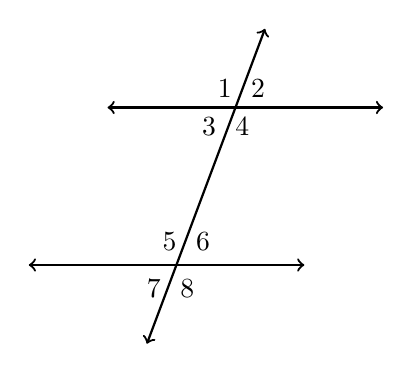
\begin{tikzpicture}[scale=1]
      \draw [<->, thick] (3.5,2)--(7,2);
      \draw [<->, thick] (2.5,0)--(6,0);
      \draw [<->, thick] (4,-1)--(5.5,3);
      \node at (4.5,0.3) [left]{$5$};
      \node at (4.5,0.3) [right]{$6$};
      \node at (4.3,-0.3) [left]{$7$};
      \node at (4.3,-0.3) [right]{$8$};
      \node at (5.2,2) [above left]{$1$};
      \node at (5.2,2) [above right]{$2$};
      \node at (5,2) [below left]{$3$};
      \node at (5,2) [below right]{$4$};
    \end{tikzpicture}
  \end{multicols}

\newpage
  \item Given two parallel lines and a transversal, with $m\angle 1 = 3x-10$ and $m\angle 8 = 2x + 32$. \\ Write an equation, then solve for $x$.
\begin{flushright}
  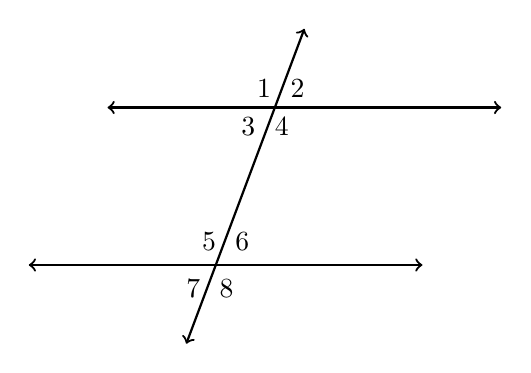
\begin{tikzpicture}[scale=1]
    \draw [<->, thick] (3,2)--(8,2);
    \draw [<->, thick] (2,0)--(7,0);
    \draw [<->, thick] (4,-1)--(5.5,3);
    \node at (4.5,0.3) [left]{$5$};
    \node at (4.5,0.3) [right]{$6$};
    \node at (4.3,-0.3) [left]{$7$};
    \node at (4.3,-0.3) [right]{$8$};
    \node at (5.2,2) [above left]{$1$};
    \node at (5.2,2) [above right]{$2$};
    \node at (5,2) [below left]{$3$};
    \node at (5,2) [below right]{$4$};
  \end{tikzpicture}
\end{flushright} \vspace{1cm}

\item Solve for $x$
  \begin{multicols}{2}
    \begin{enumerate}[itemsep=4cm]
      \item $\frac{1}{3} x-7=-4$
      \item $\frac{3}{4}x =9$
      \item $\frac{1}{2}(x-7)=12$
      \item $\frac{2}{3}(x+7)=x-4$
    \end{enumerate}
  \end{multicols} \vspace{4cm}

  \item The perimeter of a rectangle is 54 centimeters. If its length is 6 cm., what is its width?

\end{enumerate}
\end{document}